\documentclass[a4paper,10pt,english]{article}
\usepackage[utf8]{inputenc}
\usepackage[norsk]{babel}
\usepackage{amsmath,graphicx,varioref,verbatim,amsfonts,geometry}
\usepackage[usenames,dvipsnames,svgnames,table]{xcolor}
\usepackage[colorlinks]{hyperref}
\usepackage{pdfpages}
\setlength{\parindent}{0mm}
\setlength{\parskip}{1.5mm}
\usepackage{textcomp}
\usepackage{xcolor}
\usepackage{textcomp}
\usepackage{listings}
\usepackage[backend=biber]{biblatex}
\definecolor{listinggray}{gray}{0.9}
\definecolor{lbcolor}{rgb}{0.9,0.9,0.9}
\usepackage{xparse}
\renewcommand{\thesubsection}{\alph{subsection}}
\usepackage{titling}
\setlength{\droptitle}{-4em}
\addtolength{\hoffset}{-0.5in}
\addtolength{\textwidth}{0.75in}
\addtolength{\voffset}{-.5in}
\addtolength{\textheight}{1.75in}

\NewDocumentCommand{\codeword}{v}{%
\texttt{\textcolor{blue}{#1}}%
}

\lstset{
 backgroundcolor=\color{lbcolor},
 tabsize=4,
 rulecolor=,
 language=matlab,
 basicstyle=\scriptsize,
 upquote=true,
 aboveskip={1.5\baselineskip},
 columns=fixed,
 showstringspaces=false,
 extendedchars=true,
 breaklines=true,
 prebreak = \raisebox{0ex}[0ex][0ex]{\ensuremath{\hookleftarrow}},
 frame=single,
 showtabs=false,
 showspaces=false,
 showstringspaces=false,
 identifierstyle=\ttfamily,
 keywordstyle=\color[rgb]{0,0,1},
 commentstyle=\color[rgb]{0.133,0.545,0.133},
 stringstyle=\color[rgb]{0.627,0.126,0.941},
}

\addbibresource{bib.bib}
\title{Bernt Jonas Fløde
}
\author{Project 3 Computational Physics
}
\begin{document}
\maketitle

\section*{Introduksjon}
Dette projektet tar sikte på å simulere planetenes og
Solas baner i Solsystemet ved hjelp av den forlengse
Euler-metoden og Verlet-integrasjon. Metodene sammenlignes,
og vi ser hva ulike tidssteg gjør for nøyaktigheten. Vi
finner også ut hvor stor innvirkning det har å anta at
Sola står stille i Solsystemets massesentrum. Til slutt
ser vi litt på den relativistiske effekten på Merkurs bane.

\section*{Metode}
\subsection*{Fysikk}
Til å finne planetbanene brukes den klassiske
newtonske ligninga for gravitasjonell akselerasjon:
\[
a_G= \frac{GM_{\odot}}{r^2},
\]
der $M_{\odot}$ er Solas masse, $G$ er
gravitasjonskonstanten og $r$ er avstanden fra Sola til
himmellegemet som skal få akselerasjonen sin utregnet.
Formelen kan også brukes for å regne ut
tyngdeakselerasjonen fra hvilket som helst himmelegeme
på et annet, ved å bytte ut solmassen med massen til det
legemet som er kilde til gravitasjonsfeltet.

For å gjøre uttrykket relativistisk, gjøres det en liten
endring i uttrykket ved å ta med en ekstra faktor:
\[
a_G = \frac{GM_\mathrm{\odot}}{r^2}\left[1 + \frac{3l^2}{r^2c^2}\right]
\]

I en del av prosjetet skal det demonstreres sirkulære planetbaner, og for å
finne dette brukes det at sentripetalakselerasjonen skal være lik gravitasjonell
akselerasjon. Utregninga går slik:
\[
a_G = v^2 / r = G M_mathrm{\odot} / r^2
v = (G M_mathrm{\odot} / r)^{0.5}
\]

For å nå unnslippingshastighet, må kinetisk energi være minst like stor som
negativ potensiell energi. Dvs.
\[
1/2 M_{planet} v^2 = G M_mathrm{\odot} M_{planet} / r
v^2 = 2 G M_mathrm{\odot} / AU
v = (2 / G M_mathrm{\odot} / AU)^{0.5}
\]
der AU er en astronomisk enhet.

I programmet escape\_velocity.py er det lagd en animasjon som viser en planet
som akkurat har unnslippingshastigheten, samt den samme banen der
gravitasjonsloven er justert slik at 2-eksponenten har forskjellige verdier
mellom 2 og 3.

\subsection*{Programmering}
Med forlengs Euler metoden enkel. Først regnes akselerasjonen
for et gitt tidspunkt ut, så ganges den med et gitt tidssteg,
og med dette har vi funnet hastighetsendringa. Tilsvarende
gjøres for posisjonsendringa, ved å gange hastighet med
tidssteget. I kodeform kan dette skrives
\begin{lstlisting}
for (i = 0; i < N; i++)
    v[i+1] = v[i] + dt * a_G(r[i])
    r[i+1] = r[i] + dt * v[i]
\end{lstlisting}
der v er hastighetene, r er posisjonene for hver gitte
tidsindeks i, N er antall elementer i listene, dt er
tidssteget og $a_G$ er gravitasjonens akselerasjon.

Verlet-integrasjon virker annerledes, og her regnes i
utgangspunktet bare posisjonen ut. Her gis den bare i
kodeform:
\begin{lstlisting}
current_x = r[0] + v[0]*dt + 0.5*a_G(x[0])*dt**2
for (i = 0; i < N; i++):
    next_x = 2*current_x - prev_x + a_G(current_x)*dt**2
    prev_x = current_x
    current_x = next_x
    x[i] = current_x
\end{lstlisting}
For å finne hastighetene, må vi her derivere posisjonen
numerisk:
\begin{lstlisting}
v[i] = (r[i+1] - r[i-1]) / (t[i+1] - t[i-1])
\end{lstlisting}
der t er tidspunktet for en gitt tidsindeks i.

I begge tilfellene er det en forutsetning av vi kjenner
startposisjon r[0] og starthastighet v[0].

\subsection*{Datakilde}
Data for himmelegemenes startposisjon og -hastighet
hentes fra NASA: https://ssd.jpl.nasa.gov/horizons.cgi#top

\section*{Resultat}
\begin{figure}
    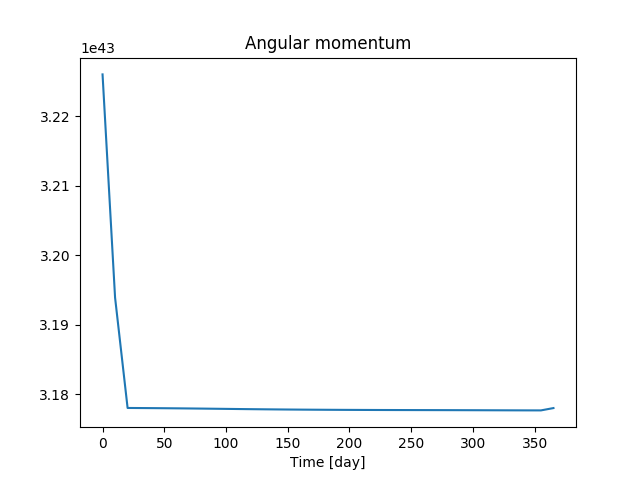
\includegraphics[width=0.5\textwidth]{3c_angular_momentum.png}
    \caption{}
    \label{fig:3cam}
\end{figure}
\begin{figure}
    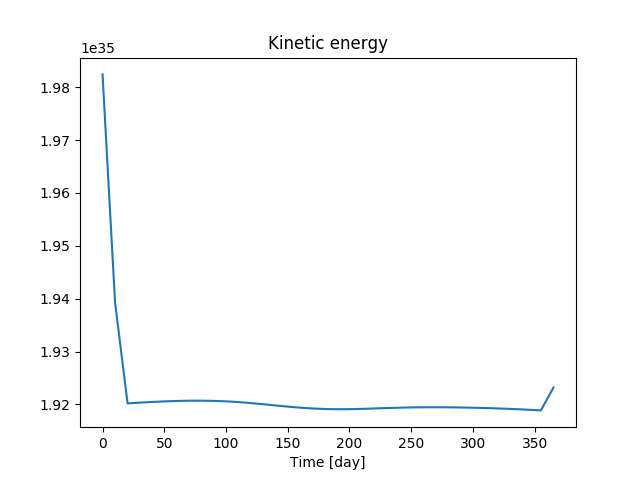
\includegraphics[width=0.5\textwidth]{3c_kinetic_energy.png}
    \caption{}
    \label{fig:3cke}
\end{figure}
\begin{figure}
    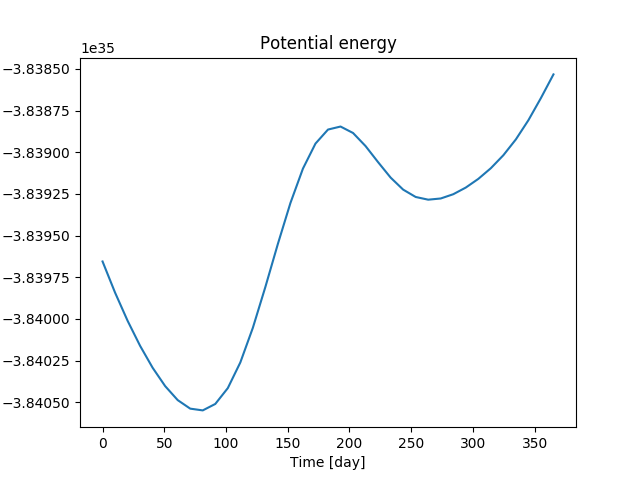
\includegraphics[width=0.5\textwidth]{3c_potential_energy.png}
    \caption{}
    \label{fig:3cpe}
\end{figure}
I figur \ref{fig:3cam}, \ref{fig:3cke} og \ref{fig:3cpe} kan vi se at både
drivmoment (eng: angulat momentum), kinetisk energi og potensiell energy ligger
stabilt sett utfra tallene på y-aksen. Dette gjelder altså for tilnærmet
sirkulær planetbane.

Når det gjelder FLOP (flyttallsoperasjoner), viser en rask telling at dette er
6 for framlengs Euler og 5 for Verlet, for hvert iterasjon. Hvis vi tar med
hastighetsutregningen med Verlet blir det derimot 9 for Verlet.
\end{document}
\grid
